\chapter*{Introduction}
\addcontentsline{toc}{chapter}{Introduction}

Accurate vehicle speed estimation plays a critical role in modern automotive systems, contributing to various functionalities such as tire slip calculation, advanced driver-assistance systems (ADAS), intelligent transportation systems (ITS), and autonomous driving technologies. Conventionally, the measurement of vehicle speed has been accomplished through two primary methods: direct measurement via wheel speed sensors or indirect derivation using GPS data. However, it must be acknowledged that these methodologies are not without their limitations. The functionality of wheel speed sensors can be compromised by factors such as wheel slip or defects in the sensor itself. Concurrently, the reliability of GPS signals is often compromised in specific environments, including tunnels, urban canyons, and dense forests.

In this context, the Controller Area Network (CAN) bus, which facilitates communication between electronic control units (ECUs) in vehicles, offers a promising alternative source of information for estimating vehicle speed. The CAN bus transmits various sensor readings and control signals continuously, with many of these signals being correlated with vehicle dynamics. The utilization of these signals for speed estimation has the potential to enhance system robustness, particularly in scenarios where traditional methods are rendered ineffective.

The advent of artificial intelligence (AI) has led to a surge in the utilization of data-driven methodologies for addressing intricate estimation challenges. Artificial intelligence (AI) models, particularly those designed for time-series data, such as recurrent neural networks (RNNs), are well-suited to capture the temporal dependencies and nonlinear relationships inherent in CAN signals. When trained effectively, these models can provide real-time, accurate estimations of vehicle speed based solely on CAN data.

This thesis explores the development and validation of AI-based models for real-time vehicle speed estimation using CAN signal data from a passenger car. The estimation performance is evaluated against GPS measurements, which serve as ground truth. Moreover, the study explores hybrid approaches that integrate artificial intelligence (AI) with conventional filtering methods, with the objective of combining the strengths of both paradigms. The enhancement of the reliability and accuracy of speed estimation contributes to the development of safer and more intelligent vehicle systems.

\chapter{Vehicle speed}

\section{Defining Vehicle Speed}

The speed of an arbitrary point in space is defined as the magnitude of the velocity vector of that point, that is considered in the inertial reference frame ($\mathcal{R}_{[x_0, y_0, z_0]}$, later denoted as $\mathcal{R}_0$ for simplicity). The velocity vector can be written as the time derivative of the position vector, where the position vector points from the origin of the inertial reference frame to the chosen moving point in space. However, when considering a moving vehicle in the same space, a relatively constrained set of points has to be considered instead of one moving point. In order to use the previously mentioned formula for determining the speed of the vehicle, one point has to be chosen on the vehicle that will represent the whole. This will be the center of gravity (CoG) that is the average location of the weight of the vehicle. With this in mind the vehicle speed can be determined as follows:
\begin{equation}
    v_{CoG} = \left\| [\textbf{v}_{CoG}]_{\mathcal{R}_0} \right\| = \left\| \frac{d [\textbf{r}_{CoG}]_{\mathcal{R}_0}}{dt} \right\|, 
\end{equation}
where $v_{CoG}$ is the vehicle speed, $[\textbf{v}_{CoG}]_{\mathcal{R}_v}$ is the velocity vector of the CoG in the inertial reference frame and $[\textbf{r}_{CoG}]_{\mathcal{R}_0}$ is the position vector of the CoG in the inertial reference frame. This way the velocity and the position vectors can be expressed in a 3 dimensional space as:
\begin{itemize}
    \item position vector: $[\textbf{r}_{CoG}]_{\mathcal{R}_0} = \begin{bmatrix} r_x \\ r_y \\ r_z \end{bmatrix}_{\mathcal{R}_0}$
    \item velocity vector: $[\textbf{v}_{CoG}]_{\mathcal{R}_0} = \begin{bmatrix} v_x \\ v_y \\ v_z \end{bmatrix}_{\mathcal{R}_0}$
\end{itemize}

As the moving vehicle in space is considered as a 3 dimensional body, the orientation of it can be described with a body-fixed reference frame denoted by $\mathcal{R}_{[x_v, y_v, z_v]}$ (later denoted by $\mathcal{R}_v$ for simplicity), where $x_v$ points forward along the vehicle frame's longitudinal axis, $y_v$ points sideways to the left along the lateral axis and $z_v$ points upwards to complete the right-handed coordinate system. Let this coordinate system be placed in the CoG of the vehicle. With the help of this body-fixed coordinate system the previously determined velocity vector ($[\textbf{v}_{CoG}]_{\mathcal{R}_0}$) can be expressed in the body-fixed reference frame with the help of the rotational transformation matrix $T_{\mathcal{R}_0 \rightarrow{} \mathcal{R}_v}$ between the two reference frames. The rotational transformation matrix can be obtained from the rotational matrices around the three axes, namely $x_0$, $y_0$ and $z_0$.
The angles of rotation around the axes are the following:
\begin{itemize}
    \item angle of rotation around axis $x_0$: roll - $\phi$
    \item angle of rotation around axis $y_z$: pitch - $\theta$
    \item angle of rotation around axis $z_0$: yaw - $\psi$
\end{itemize}
From here the transformation matrix is as follows:
\begin{equation}
    T_{\mathcal{R}_0 \rightarrow{} \mathcal{R}_v} = R_z(\psi) \cdot R_y(\theta) \cdot R_x(\phi) 
\end{equation}

\FloatBarrier
\begin{figure}[h]
    \centering
    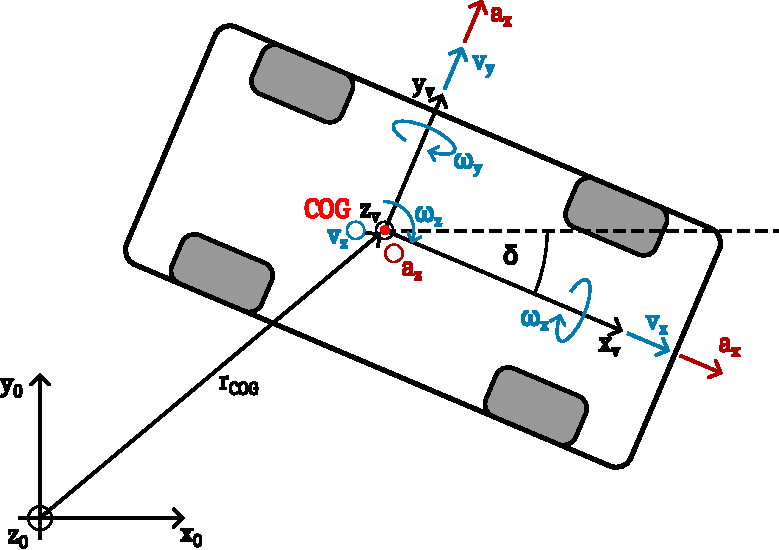
\includegraphics[width=0.9\textwidth]{images/vehicle_speed.pdf}
    \caption{Vehicle speeds}
    \label{fig:geom_veh_speed}
\end{figure}
\FloatBarrier

\section{Measurements for determining vehicle speed}
\label{sec:Measurements}

There are various ways to determine the speed of the vehicle. In this section the focus is on exploring these different ways and analyzing them. 

\subsection{Engine speed}

The first way is calculating the wheel and vehicle speed from the rotational speed of the engine \cite{engine_speed}. It is a rather theoretical calculation but it gives a simplified overview how the engine is connected to the wheels through the gearbox and the differential. The setup can be seen on Figure \ref{fig:egine_speed}.
\FloatBarrier
\begin{figure}[h]
    \centering
    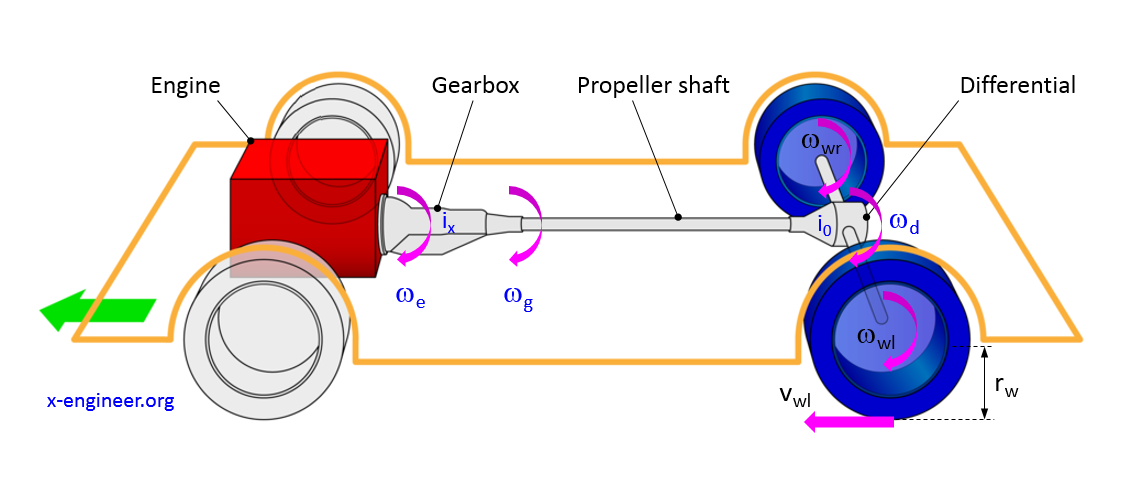
\includegraphics[width=0.9\textwidth]{images/Vehicle-longitudinal-powertrain-diagram-speed-calculation.png}
    \caption{Calculating vehicle speed from engine speed \cite{engine_speed}}
    \label{fig:egine_speed}
\end{figure}
\FloatBarrier
The formula for determining the vehicle speed is the following:
\begin{equation}
    v_v = \frac{N_e \cdot \pi \cdot r_{\omega}}{30 \cdot i_x \cdot i_0} \left[ \frac{m}{s} \right],
\end{equation}
where $N_e$ [rpm] is the engine speed, $r_{\omega}$ [m] is the wheel radius, $i_x$ [-] is the gear ratio of the engaged gear and $i_0$ [-] is the gear ratio of the differential. 

The main advantage of this method comes from its simplicity. Based on a one measured data, that is the engine shaft's rotational speed ($N_e$), the longitudinal vehicle speed can be determined. Contrary to this it can only give a estimate due to the simplifications it considers. It doesn't take in account the slip in the clutch between the gearbox and the engine shaft, the longitudinal and lateral slip of the tires, the difference in speed of the left and right wheels in case of traveling in a curve, the case when the gearbox and the engine are detached while the vehicle is being in neutral (gear 0) and when the wheels are locked but the vehicle is still motion. Considering the points mentioned above, this method could be used in highway driving where the vehicle travels with constant high speed on a straight path with little curvature. 

\subsection{Wheel speed}

Following the previous method where the measured unit was the rotational speed of the engine's shaft, here the shift goes to measuring the rotational speed of the vehicle's wheel. This is done by a speedometer. The first speedometer is credited to Josip Belušić \cite{Josip_Belusic}. His invention in 1888 was based on the electromagnetic induction which worked the following way. A flexible rotating cable is connected to the vehicle wheel's rotating shaft via a friction disk or a pair of gears that translates the rotational motion to a disk shaped magnet. This rotating magnet creates a fluctuating magnetic field which induces a rotating movement in the speed cup that surrounds the magnet. However the speed cup's movement is limited by a spring. This spring will allow greater rotation when greater torque applies to the speed cup that is in the case of faster rotation from the magnet. The needle that showed the speed of the vehicle is linked to the speed cup. This way the needle moved proportionally to the speed of the vehicle \cite{speedometer}. Later this principle was patented by Otto Schulze in 1903 \cite{speedometer_patent_Otto} and Joseph W Jones in 1904 \cite{speedometer_patent_Joseph}. Both of the patents share the same principle.  
\FloatBarrier
\begin{figure}[ht]
    \centering
    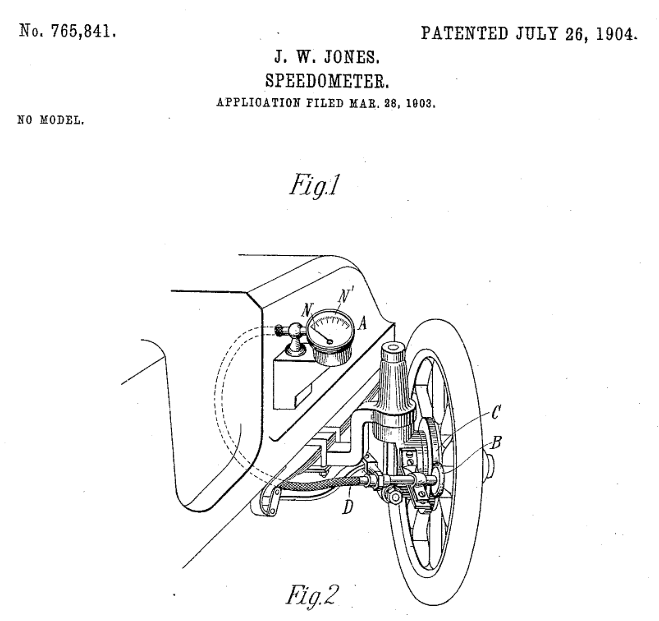
\includegraphics[width=0.6\textwidth]{images/speedometer_patent.png}
    \caption{Speedometer patented by Joseph W Jones in 1904 \cite{speedometer_patent_Joseph}}
    \label{fig:speedometer_patent}
\end{figure}
\FloatBarrier
The rather mechanical method described above was in use for several decades but it has multiple downsides: wear of the elements due to the mechanical connections, uncertainty coming from the mechanical measurement method and the fact of having the speed from only one wheel. To compensate the points mentioned before, electric wheel speed sensors were introduced to enhance the precision of the measurements. There are two types of electronic wheel speed sensors: passive and active. 

The principle of the passive wheel speed sensor is the following. A toothed reluctant ring is mounted on the rotating wheel. Above this ring a variable reluctance (VR) sensor is placed. When the wheel starts to rotate each tooth changes the magnetic flux through the coil of the sensor which induces an alternating voltage signal. The frequency of this analog sine wave is proportional to the rotational speed. However, the active wheel speed sensor uses a semiconductor magnetic sensor (Hall or magneto-resistive sensor) and a magnetic encoder ring attached to the rotating wheel. As the ring rotates, the magnetic field changes are detected by the magnetic sensor. These changes are then converted to square wave digital signals \cite{wheel_speed_sensors}. The active sensors can overall provide a more precise measurement than the passive sensors.
\FloatBarrier
\begin{figure}[htbp]
    \centering
    \begin{minipage}{0.45\textwidth}
        \centering
        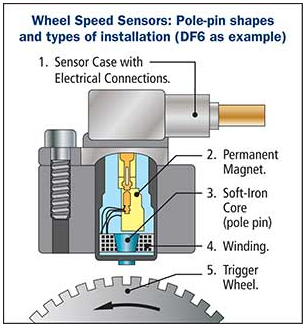
\includegraphics[width=\linewidth]{images/passive_wheel_speed_sensor.png}
    \end{minipage}
    \hfill
    \begin{minipage}{0.45\textwidth}
        \centering
        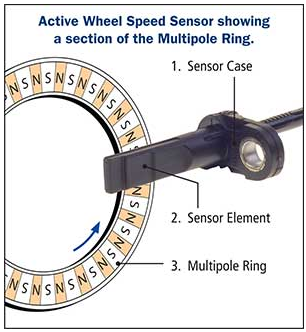
\includegraphics[width=\linewidth]{images/active_wheel_speed_sensor.png}
    \end{minipage}
    \label{fig:wheel_speed_sensors}
    \caption{Passive (left) and active (right) wheel speed sensors from \cite{wheel_speed_sensors}}
\end{figure}
\FloatBarrier

In the case of these wheel speed sensors, the output is a rotational speed. From this rotational speed the ground speed of the specific wheel can be determined with the help of the diameter of the wheel. This measurement can be done for all the wheels, which will serve as an input for later discussed estimator algorithms.


\subsection{Inertial Measurement Unit}

The inertial measurement unit (IMU) can also provide relevant measurement data to determine the vehicle speed. An IMU consist of a set of linear accelerometers and gyroscopes to determine the acceleration along and the rotational rate around the longitudinal, lateral and vertical axes. This gives two vectors: acceleration $\textbf{a}$ and angular velocity vector $\boldsymbol{\omega}$ in the body fixes coordinate system:
\begin{equation}
    \textbf{a} = \begin{bmatrix}
        a_x \\ a_y \\ a_z 
    \end{bmatrix}
    \text{ and }
    \boldsymbol{\omega} = 
    \begin{bmatrix}
        \omega_x \\ \omega_y \\ \omega_z
    \end{bmatrix}
\end{equation}
Before calculating the velocity, the gravitational vector has to be deducted from the measured acceleration vector that can be done with the help of the angular velocity vector. From here, as the velocity vector's time derivative equals the acceleration vector, the velocity can be derived by an integral:
\begin{equation}
    \textbf{v}(t) = \textbf{v}(t_0) + \int_{t_0}^{t} \textbf{a}(\tau) d(\tau)
\end{equation}
It is important to mention here that this measurement method is not robust by itself. Apart from setting the initial velocity of the vehicle, the biases in the accelerometers lead to integration drift that accumulates into large errors over time. To mitigate this issue this method has to be combined with other velocity measurements and estimators.

\subsection{Global Navigation Satellite System}
\label{subsec:GNSS}

Global Navigation Satellite System (GNSS) refers to any constellation that provides global positioning, navigation and timing services. The currently available GNSS systems in Europe are GPS, Galileo, Glonass and BeiDou \cite{GNSS}. 

The velocity of the vehicle can be obtained by exploiting the raw Doppler, the carrier phase or the pseudorange measurements with a GNSS receiver. These measurements are the following: 
\begin{itemize}
    \item Raw Doppler (RD) measurement:
    \begin{itemize}
        \item The RD measurement captures how much does the frequency of the signal change between transmitting and receiving.
        \begin{equation}
            D = f_{transmitted} - f_{received}
        \end{equation}
        \item The Doppler shift $D$ is related to the change of the distance between the satellite and the receiver. From the Doppler shift the range rate $\dot\rho$ can be determined that is the radial velocity $v_r$ along the range between the satellite and the receiver.
        \begin{equation}
            \dot\rho = v_r = \lambda \cdot D = \dot\rho + c
        \end{equation}
    \end{itemize}
    \item Carrier phase measurement:
    \item Pseudorange differentiation:
\end{itemize}

\FloatBarrier
\begin{figure}[htbp]
    \centering
    \begin{minipage}{0.45\textwidth}
        \centering
        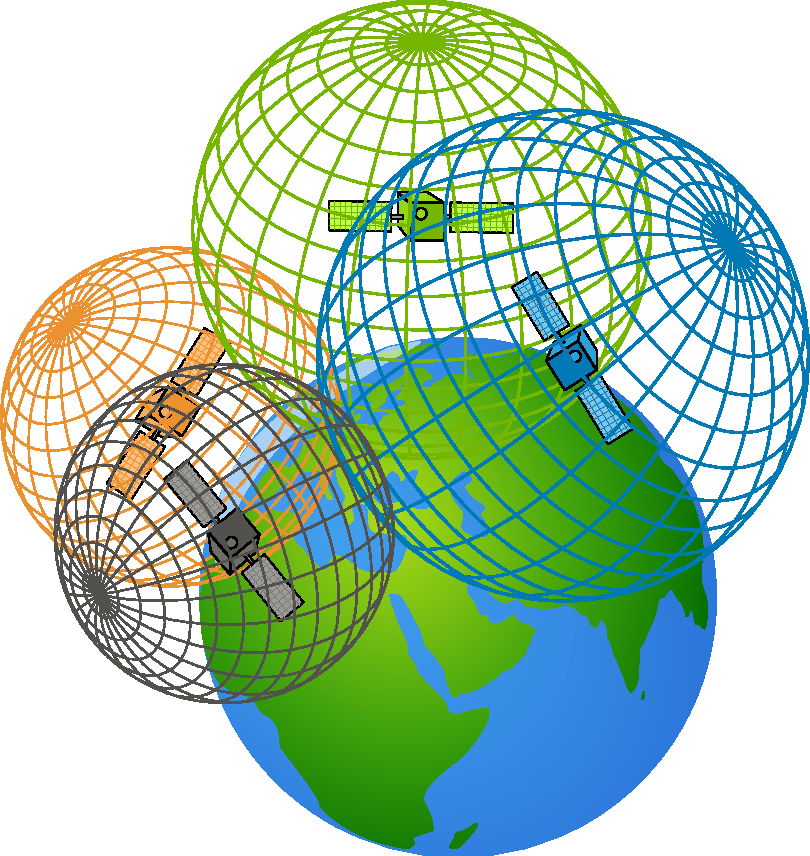
\includegraphics[width=\linewidth]{images/trilateration.pdf}
    \end{minipage}
    \hfill
    \begin{minipage}{0.45\textwidth}
        \centering
        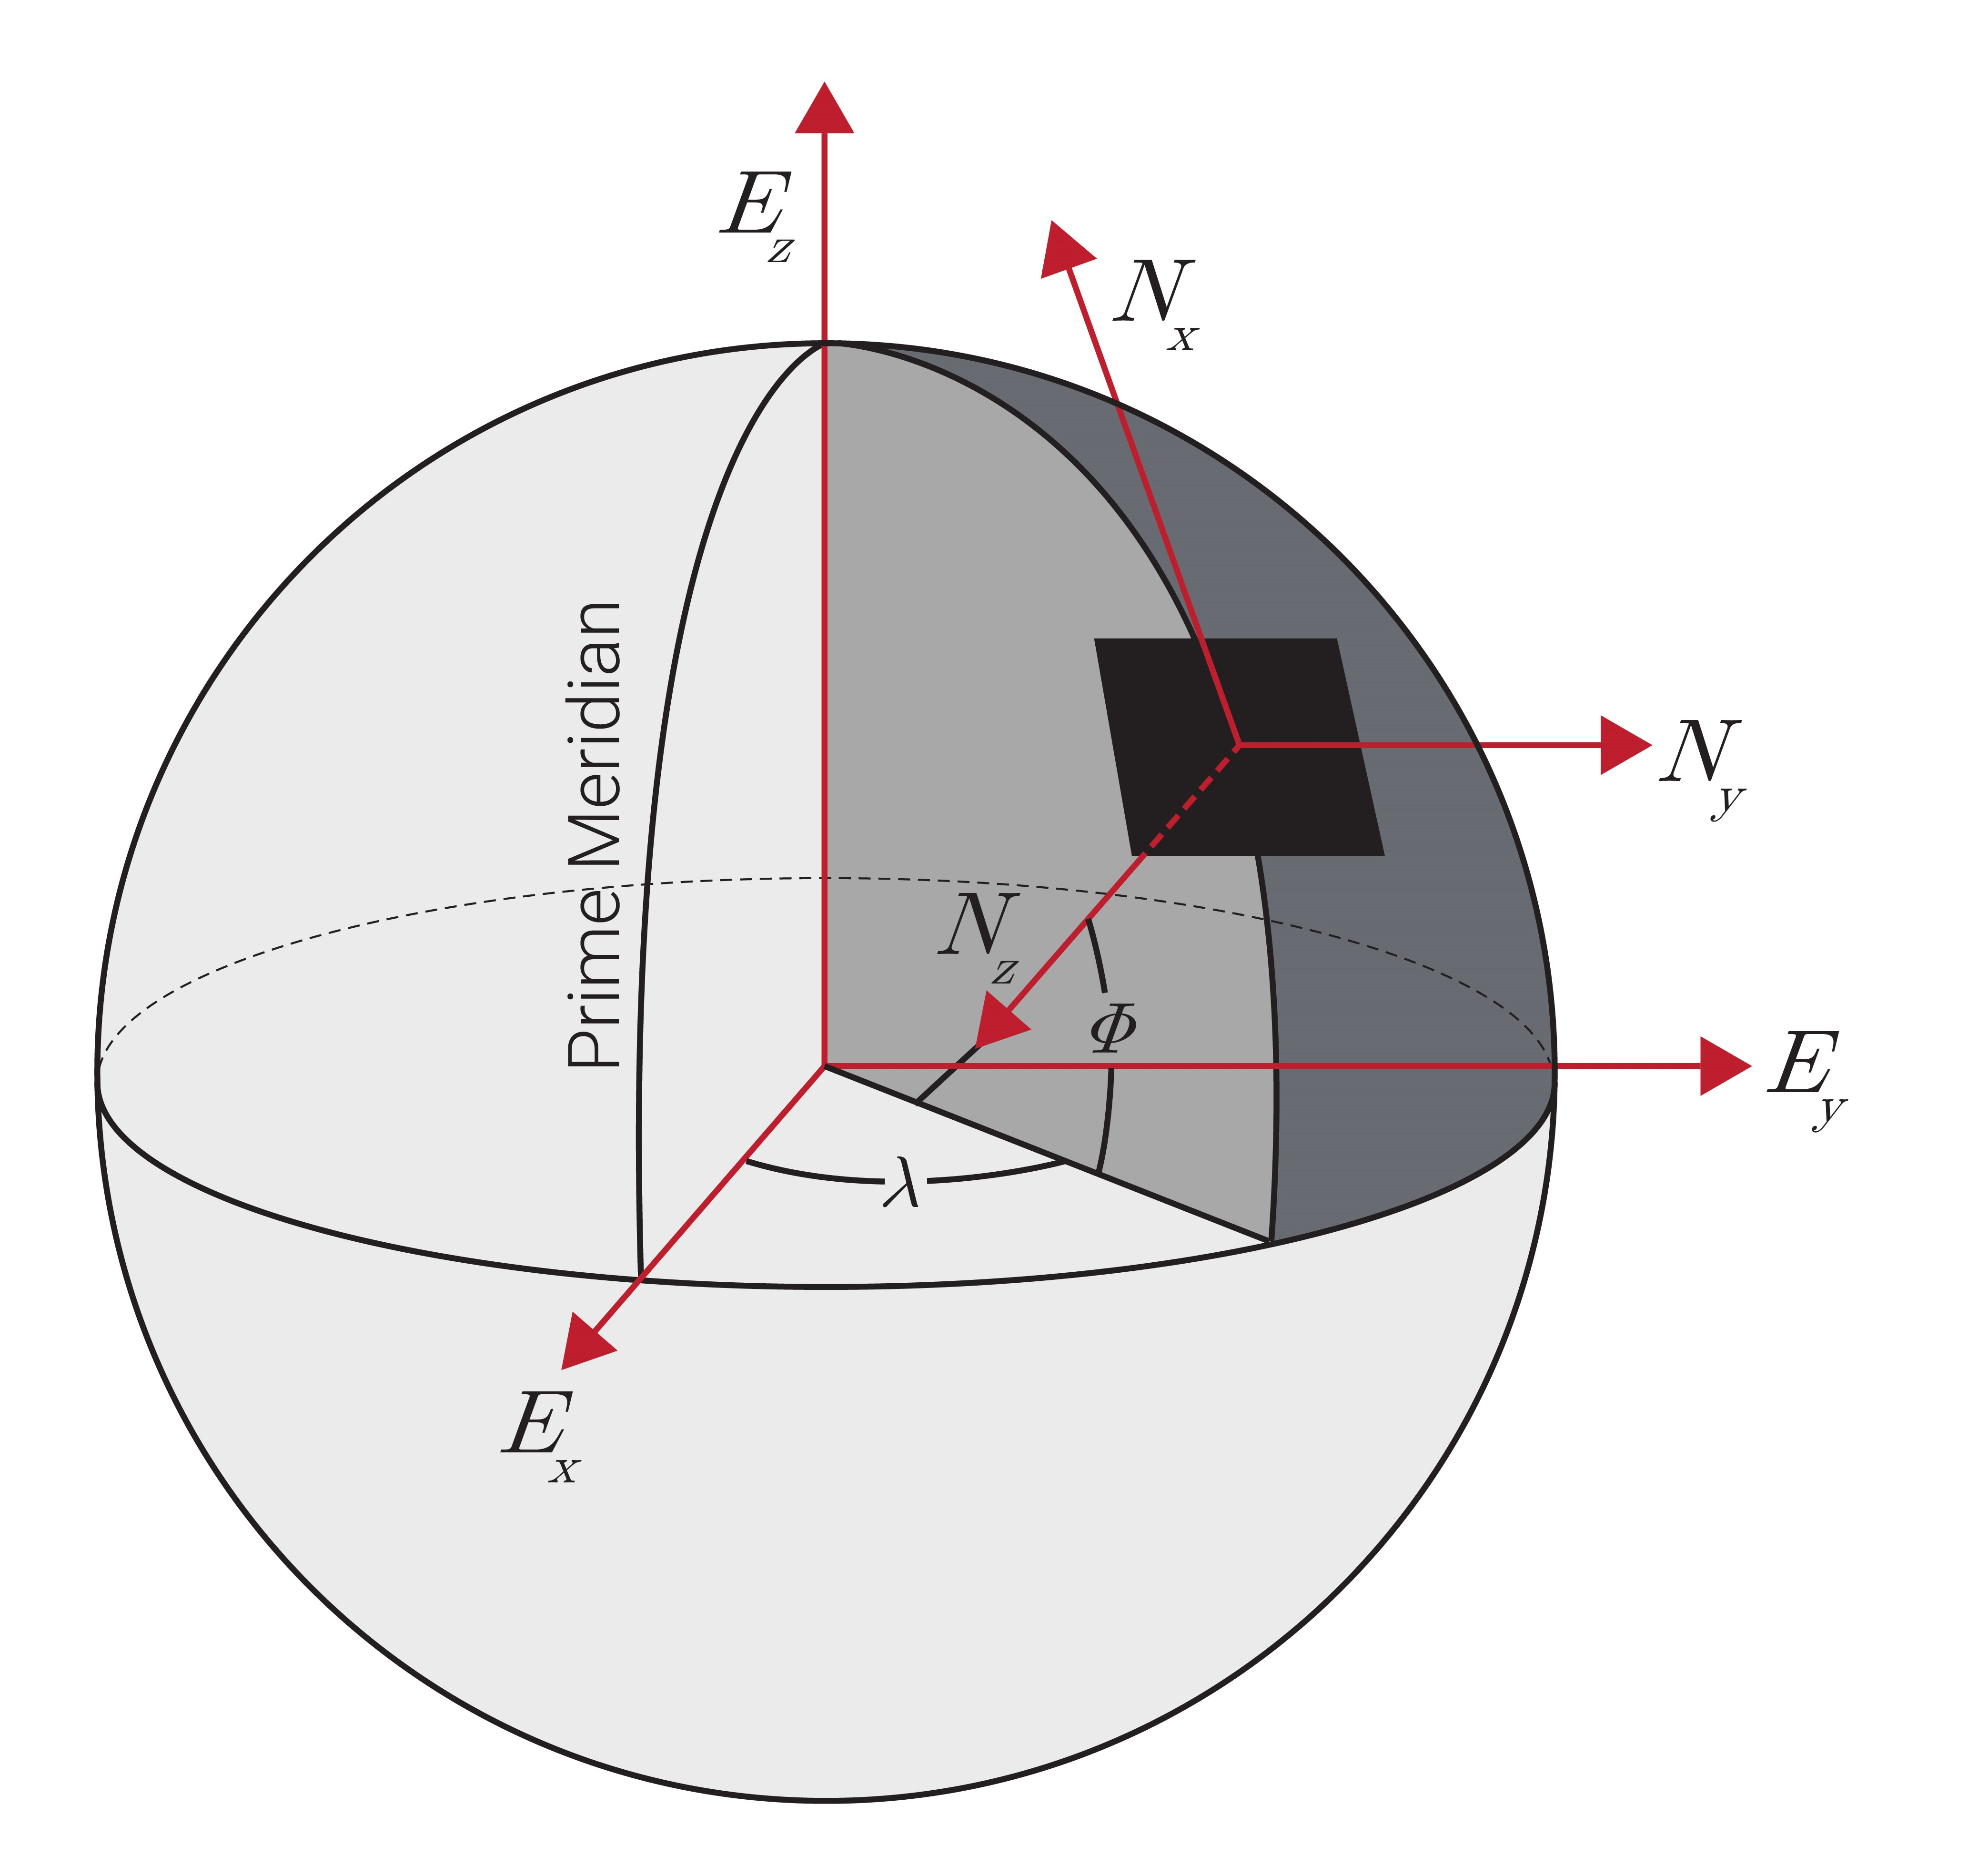
\includegraphics[width=\linewidth]{images/ecef.jpg}
    \end{minipage}
    \label{fig:GNSS}
    \caption{Trilateration (left) from \cite{gps-satellites-trilateration} and ECEF coordinate system (right) from \cite{ECEF_coordinate_sys}}
\end{figure}
\FloatBarrier

\section{Estimating vehicle speed}

\subsection{Accelerometer and speedometer}
The simplest method to estimate the vehicle speed is to take the measurements from the speedometers at all the wheels. The longitudinal speed of each wheel can be determined from the rotational speed data from the sensors. These values then can be transformed into the CoG of the vehicle. There the transformed longitudinal velocities can be compared and the largest one can be chosen.
\begin{equation}
    v_{CoG} = max[v_{FR}; v_{FL}; v_{RR}; v_{RL}],
\end{equation}
where $v_{FR}$, $v_{FL}$, $v_{RR}$and $v_{RL}$ are the transformed velocity values from each wheel. 

Another simple algorithm for vehicle speed estimation is presented in \cite{lit_simple_veh_speed}. Here the vehicle speed is determined by the measurements from the IMU's longitudinal accelerometer and the wheel speed sensors. The formula that estimates the speed is described as follows:
\begin{equation}
    v_{CoG}(k) = v_{simple}(k_{nobrake}) + \sum_{i=k_{nobrake}}^{k} a_{meas}(i)\cdot dt,
\end{equation}
where the $k$ is the time step counter, $k_{nobrake}$ is the last time index where there was no braking, $a_{meas}$ is the acceleration value form the IMU's longitudinal accelerator and $dt$ is the time sample. This method works in a way that estimation is taken apart into two categories based on whether the vehicle is barking or not. 
The simplicity comes at the price of inaccuracies. The estimator does not perform well when accelerometer offset is set and the dynamic change of the wheel radius is not implemented. An other difficulty comes from dealing with the noisy measurements from the wheel speed sensors and the IMU. 
\FloatBarrier
\begin{figure}[ht]
    \centering
    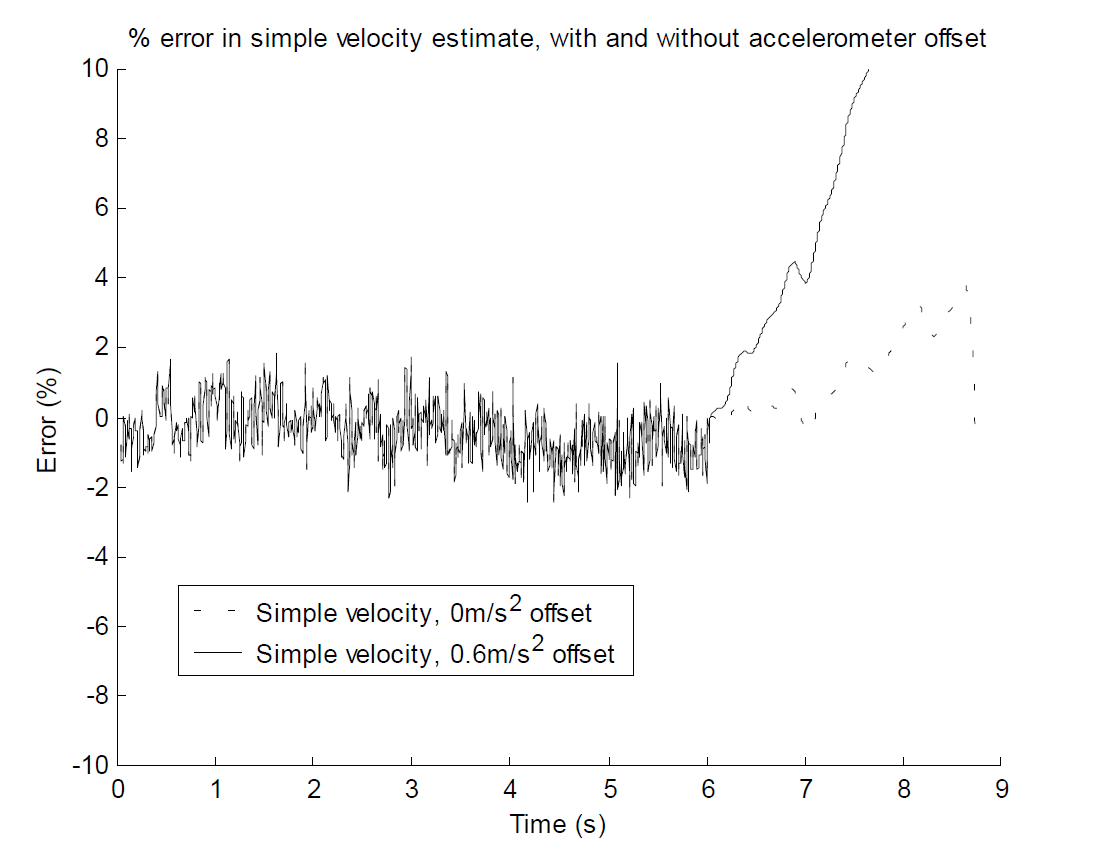
\includegraphics[width=0.6\textwidth]{images/simple_estimator.png}
    \caption{Simple algorithm for estimating vehicle speed form \cite{lit_simple_veh_speed}}
    \label{fig:simple_veh_speed_est}
\end{figure}
\FloatBarrier

\subsection{Kalman filter}
To elevate the performance of the previously described methods, a Kalman filter can be added to the system. At a high level the Kalman filter estimates the vehicle speed from noisy sensor data by iterating between the following two steps:
\begin{enumerate}
    \item Prediction
    \begin{itemize}
        \item The filter takes the last estimate and predicts the next state's longitudinal or lateral velocity based on the simple dynamic motion model.
        \item The filter provides an estimate and a uncertainty measure for the prediction.
    \end{itemize}
    \item Correction
    \begin{itemize}
        \item Based on the predicted data and the new measurement data the filter calculates an optimal blend of the two values.
        \item A posterior estimate is determined that is more accurate and less noisy than the pure measurement data. 
    \end{itemize}
\end{enumerate}
Following this structure a Kalman filter is proposed in \cite{lit_for_Kalman_fuzzy} to estimate the vehicle's speed. To enhance the accuracy of the estimator, 4 different driving situations are described with 4 different covariance matrices.
\FloatBarrier
\begin{figure}[ht]
    \centering
    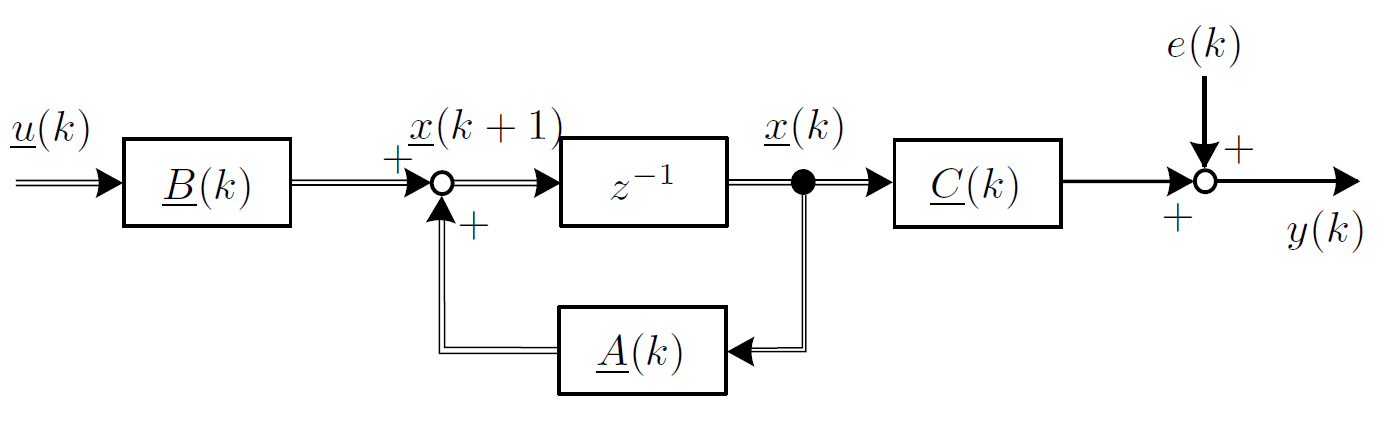
\includegraphics[width=0.6\textwidth]{images/kalman_filter.png}
    \caption{Vehicle speed estimation with Kalman filter from \cite{lit_for_Kalman_fuzzy}}
    \label{fig:kalman_filter}
\end{figure}
\FloatBarrier

To elevate the usage of Kalman filter a more sophisticated and non-linear vehicle model can be used to predict the vehicle speed. In \cite{lit_model_based_est} an Extended Kalman filter is introduced with vehicle model that runs parallel with the system itself. The overview of the filtering approach can be seen on figure \ref{fig:model_based}

\begin{figure}[ht]
    \centering
    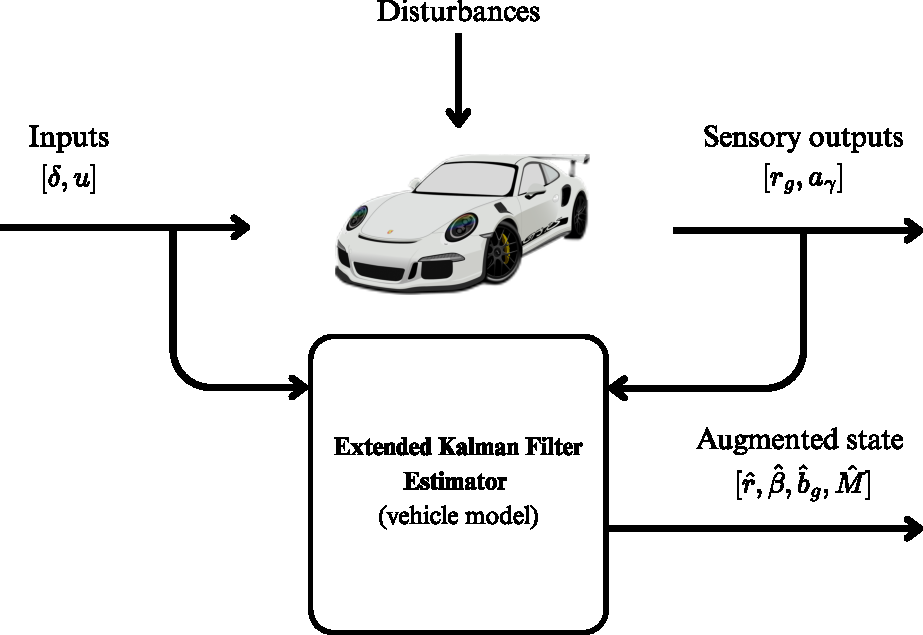
\includegraphics[width=0.8\textwidth]{images/Extended Kalman Filter Estimator (vehicle model).pdf}
    \caption{Extended Kalman filter for vehicle speed estimation from \cite{lit_model_based_est}}
    \label{fig:model_based}
\end{figure}
\FloatBarrier

\subsection{Fuzzy logic}
An other approach to estimate the vehicle speed is using fuzzy logic. Fuzzy logic offers heuristic approach to handle uncertainty and imprecision of the sensors. In \cite{lit_for_Kalman_fuzzy} a comprehensive method is described using the Fuzzy logic to determine the vehicle speed using different driving scenarios.

The main motive behind the proposed estimator is determining the weights of the sensor signal values. All the speed values coming from the senors receive a weighting factor $k_i$. The weighted average is then  formulated as follows:
\begin{equation}
    \hat v_{CoG}(k) = \frac{\sum_{i=4}^4 k_i \cdot v_{Ri,C}(k) + [\hat v_{CoG}(k-1) + T_S\cdot a_{X,C}(k)]}{\sum_{i=1}^5 k_i},
\end{equation}
where the $k_i$ weights are determined with the rules of the fuzzy logic. The overall scheme of the algorithm can be seen on figure \ref{fig:fuzzy_system}.
\FloatBarrier
\begin{figure}[ht]
    \centering
    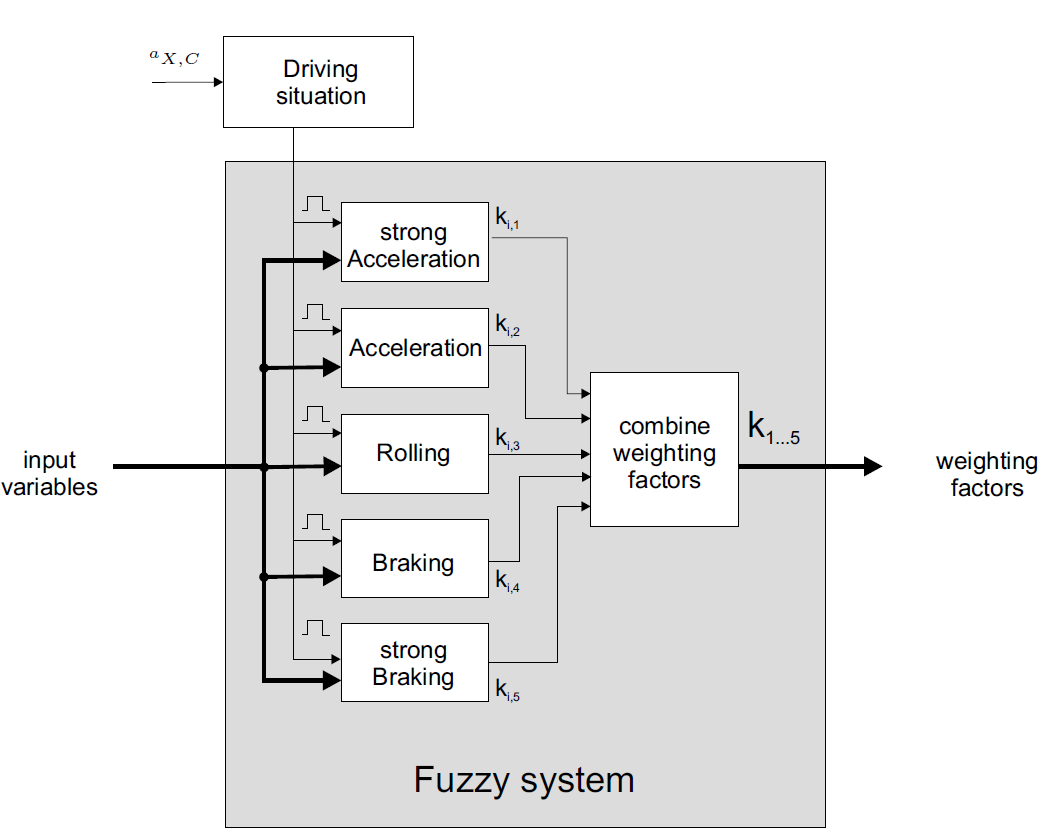
\includegraphics[width=0.8\textwidth]{images/fuzzy_logic.png}
    \caption{Vehicle speed estimation with Fuzzy logic from \cite{lit_for_Kalman_fuzzy}}
    \label{fig:fuzzy_system}
\end{figure}
\FloatBarrier

\subsection{GNSS}
There are multiple algorithms to determine the velocity of the vehicle using the GNSS system. In article \cite{GNSS_velocity_estimation} 4 algorithms are described and compared. These methods are the following: Raw Doppler (RD), Time‑Differenced Pseudorange (TDPR), Time‑Differenced Carrier Phase (TDCP) and Double‑Differenced Carrier Phase (DDCP). These algorithms were both tested in static and dynamic environments and postprocessed after the tests. 

The most accurate algorithm in dynamic environments is the RD method that utilizes the Doppler shift from the carrier phase difference of the transmitted and received signal. The measurement model can be written as:
\begin{equation}
    \lambda D = \dot \rho + c(d \dot t_R - d \dot t_S) + \dot I_{\rho} + \dot T_{\rho} + \dot \epsilon_{\rho},
\end{equation}
where $\lambda$ is the wavelength, $D$ is the Doppler shift, $\dot\rho$ is the rate of the pseudorange, $c$ is the speed of light in vacuum, $d\dot t_R$ and $d\dot t_S$ are the satellite and receiver clock drifts, $\dot I_{\rho}$ and $\dot T_{\rho}$ are the rates of change in the ionospheric and tropospheric delays and $\dot \epsilon_{\rho}$ combines the unmodeled error and observation noise. From this model the velocity of the vehicle can be determined in the global ECEF frame. The tests with this method resulted a [cm/s] level accuracy that is precise and accurate enough for driver assistance features. 

The significant advantage of this algorithm is definitely the precision that it provides and can be used to enhance the previously described estimators. The disadvantages are that the GNSS receivers are not standard in passenger and commercial vehicles leaving little space for wide-spread usage of the advantages, the 10 [Hz] sampling time is relatively low that requires some type of interpolation between the samples and that the determined velocity is not in the vehicle's body fixed frame. For determining the longitudinal and lateral velocities the heading angle is required that can be calculated if two receivers are applied to the vehicle. The last disadvantage comes from the situations when the signals from the satellites are not visible in case of driving in a tunnel or urban areas with tall buildings. 

%\subsection{Computer vision}
%Computer 

\subsection{Artificial Intelligence}
After discussing the more conventional estimators that rely on deterministic formulas for calculating the vehicle speed, let the focus be shifted to the main topic of this thesis: Artificial Intelligence (AI) for vehicle speed estimation. 

Artificial intelligence has been a greatly investigated field in the recent years for a wide range of applications. Despite the robustness and highly safety critical approach of the vehicle industry, the investigation of possible applications has been started. There are two main approaches: 
\begin{enumerate}
    \item Integrating AI algorithms to previously developed and used algorithms and models. This way an AI algorithm can be seen as a way to enhance the already developed and tested estimators.
    \item Replace the previously used algorithms with a trained AI algorithm.
\end{enumerate}
In article \cite{lit_deep_dynamics} a physics-constrained neural network (PCNN) has been introduced. This approach merges the well established and developed physical models with the advantages of a neural network (NN). Here the created network is capable of learning the coefficients of a single track vehicle model that can predict the vehicle's movement. The main advantage of this application is that by using the known dynamic and physical properties of a vehicle, the coefficients can be determined faster and more precisely than if there were no established constrains. 
\FloatBarrier
\begin{figure}[ht]
    \centering
    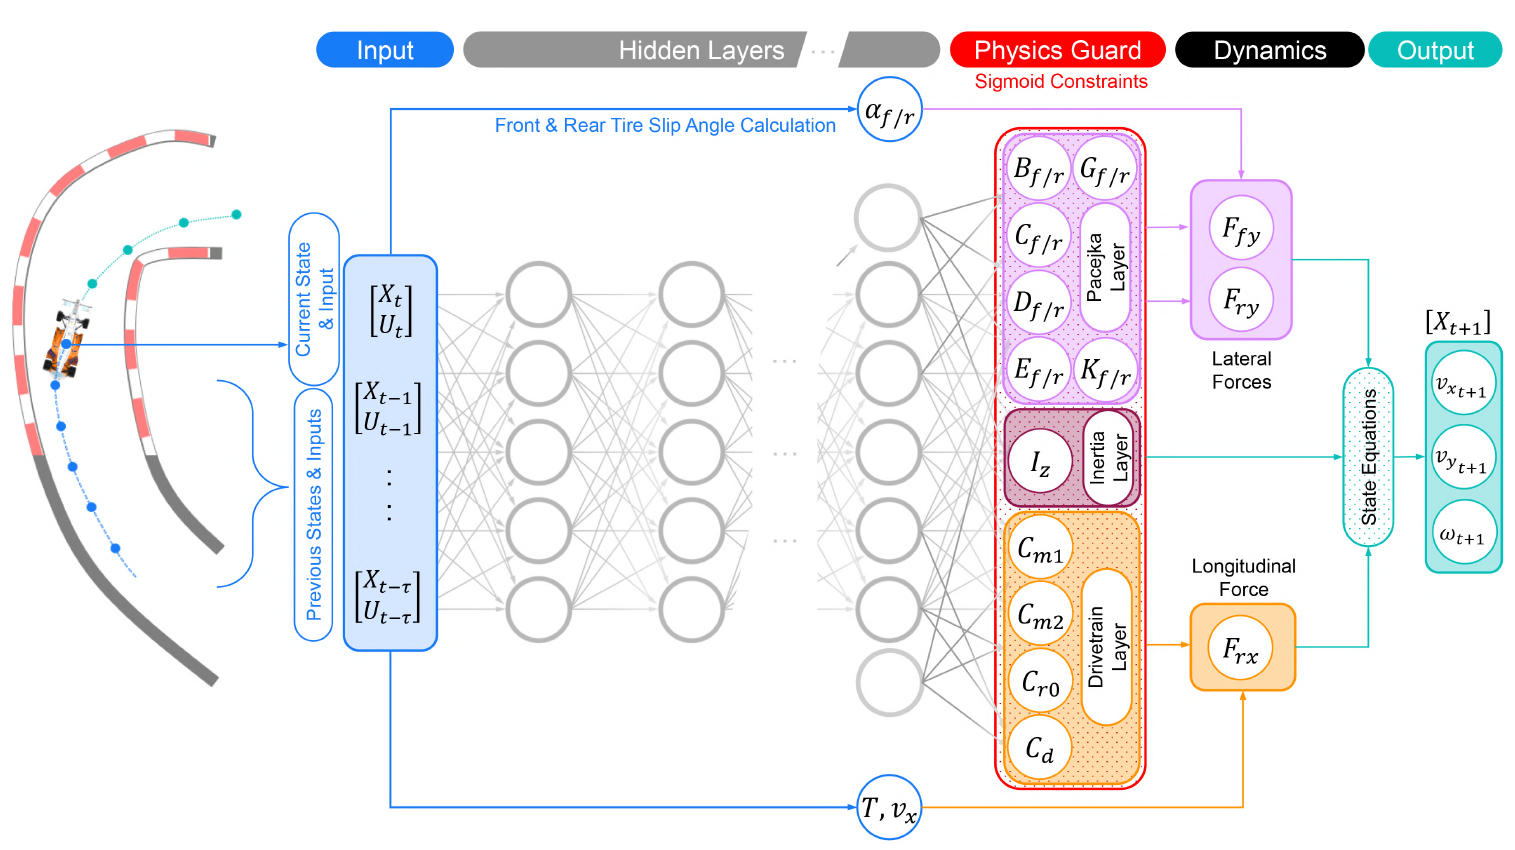
\includegraphics[width=0.8\textwidth]{images/deep_dynamics.png}
    \caption{Physics constrained neural network from \cite{lit_deep_dynamics}}
    \label{fig:deep_dynamics}
\end{figure}
\FloatBarrier
A similar approach was investigated in \cite{lit_ai_physiscs_embedded_neural_network} where a physics embedded neural network in combination of a vehicle model was developed where the previously discussed advantages were exploited. The outcome of this investigation was the performance shift from the baseline neural network model showing faster learning speed, higher accuracy and better generalization. 
\FloatBarrier
\begin{figure}[ht]
    \centering
    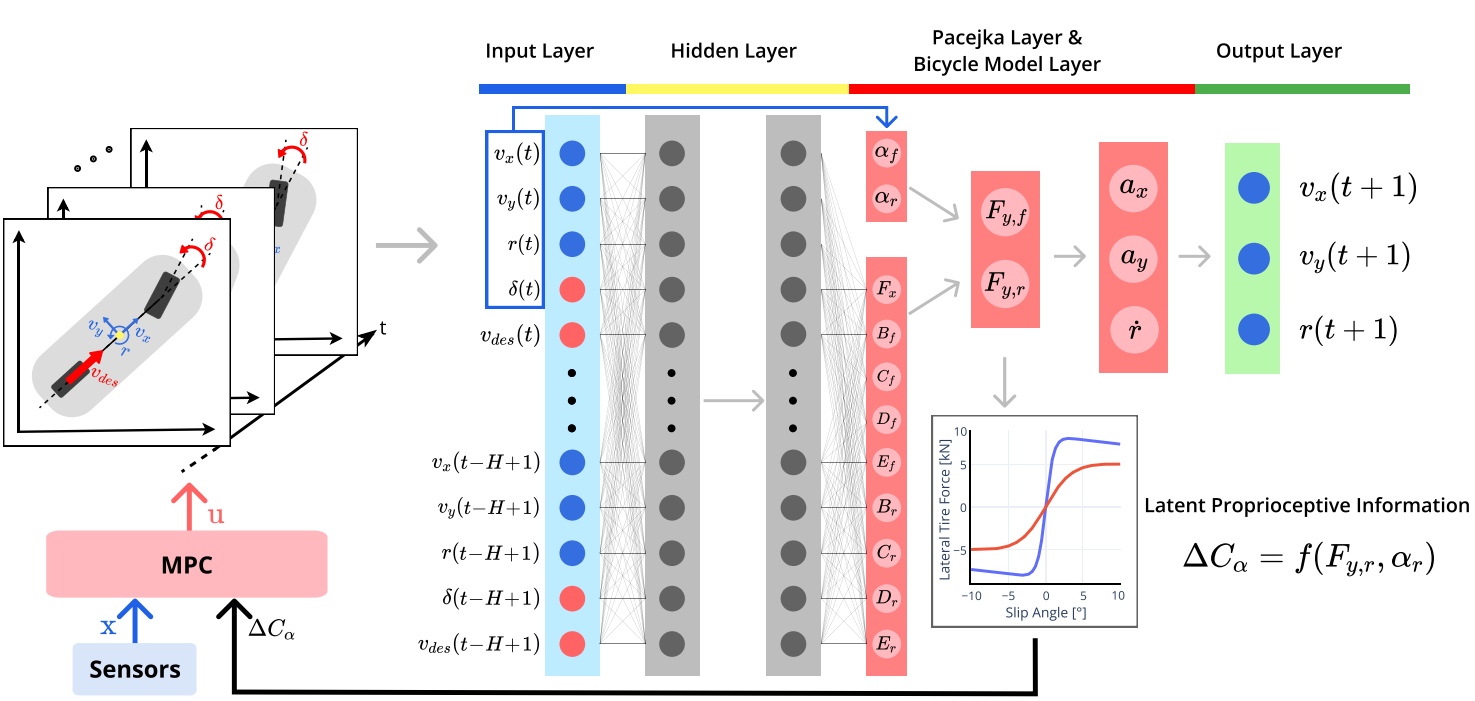
\includegraphics[width=0.8\textwidth]{images/physiscs_embedded_neural_network.png}
    \caption{Physics embedded neural network for state estimation from \cite{lit_ai_physiscs_embedded_neural_network}}
    \label{fig:physics_embedded_neural_network}
\end{figure}
\FloatBarrier

An other approach is to combine AI algorithms with Kalman filtering to enhance state estimation \cite{lit_trans_lstm}. Here a method for combining Long-Short Term Memory network (LSTM), Transformers and  Expectation-Maximization - Kalman Filter (EM-KF). This combined approach of TL-KF (Transformers, LSTM - Kalman filter) is capable of capturing long term dependencies and model time-series data. The structure of the developed model can be seen on figure \ref{fig:trans_lstm}
\FloatBarrier
\begin{figure}[ht]
    \centering
    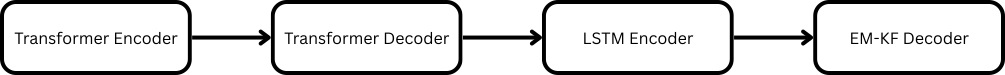
\includegraphics[width=1\textwidth]{images/Transformer Encoder.png}
    \caption{TS-KF model from \cite{lit_trans_lstm}}
    \label{fig:trans_lstm}
\end{figure}
\FloatBarrier   

\section{Conclusions}
During the literature review a comprehensive overview was presented about the used and developed vehicle speed estimators. It is visible that the well established estimators, like different model based estimators with Kalman filters have been there for longer time. In the meantime, the newly emerging field of AI has a promising future in state estimation aiding the already used estimator algortihms. 